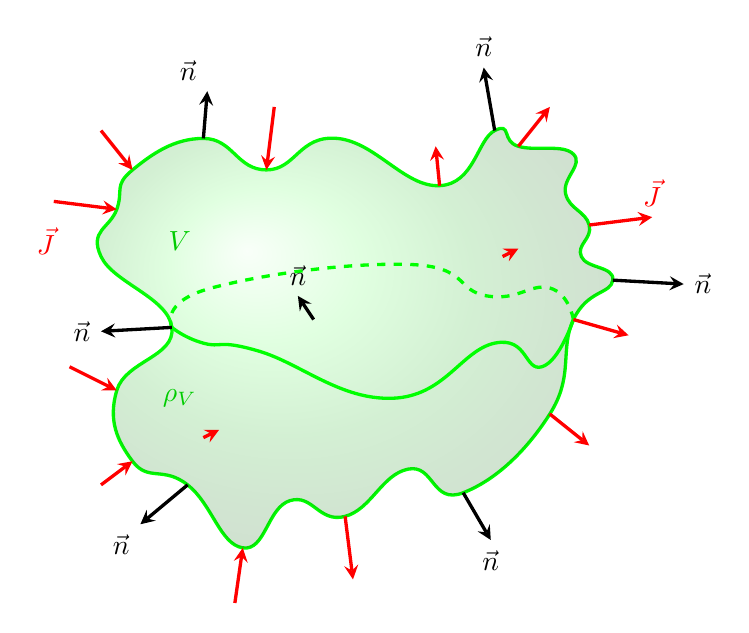
\begin{tikzpicture}[line width = 1.2pt, line join=round,x=1cm,y=1cm,>=stealth]
	% Koordinaten des Volumens
	\coordinate (a) at (3,0);
	\coordinate (b) at (3.5,0.5);
	\coordinate (c) at (3.1,0.8);
	\coordinate (d) at (3.2,1.2);
	\coordinate (e) at (2.9,1.6);
	\coordinate (f) at (3.0,2.1);
	\coordinate (g) at (2.3,2.2);
	\coordinate (h) at (2,2.4);
	\coordinate (i) at (1.3,1.7);
	\coordinate (j) at (0,2.3);
	\coordinate (k) at (-0.9,1.9);
	\coordinate (l) at (-1.7,2.3);
	\coordinate (m) at (-2.6,1.9);
	\coordinate (n) at (-2.5,1.6);
	\coordinate (o) at (-2.8,1.4);
	\coordinate (p) at (-3,0.8);
	\coordinate (q) at (-2.1,-0.1);
	\coordinate (r) at (-2.8,-0.9);
	\coordinate (s) at (-2.6,-1.8);
	\coordinate (t) at (-1.9,-2.1);
	\coordinate (u) at (-1.2,-2.9);
	\coordinate (v) at (-0.6,-2.3);
	\coordinate (w) at (0.1,-2.5);
	\coordinate (x) at (0.9,-1.9);
	\coordinate (y) at (1.6,-2.2);
	\coordinate (z) at (2.7,-1.2);
	% Volumen
	\draw [color=green] plot [smooth cycle, tension=0.8] coordinates {(a) (b) (c) (d) (e) (f) (g) (h) (i) (j) (k) (l) (m) (o) (p) (q) (r) (s) (t) (u) (v) (w) (x) (y) (z)};
	\shade [ball color=white!20!green, opacity=0.20] plot [smooth cycle, tension=0.8] coordinates {(a) (b) (c) (d) (e) (f) (g) (h) (i) (j) (k) (l) (m) (o) (p) (q) (r) (s) (t) (u) (v) (w) (x) (y) (z)};
	\draw [color=green] plot [smooth, tension=0.8] coordinates {(a) (2.6,-0.6) (2,-0.3) (0.7,-1) (-1,-0.4) (-1.7,-0.3) (q)};
	\draw [color=green, dashed] plot [smooth, tension=0.8] coordinates {(a) (2.7,0.4) (1.9,0.3) (0.9,0.7) (-1.6,0.4) (q)};
	\draw [color=green!80!black] (-2,1) node {$ V $};
	\draw [color=green!80!black] (-2,-1) node {$ \rho_\text{V} $};
	% Normalenvektoren
	\draw [->] (q) -- ++(-0.9,-0.05) node[anchor=east] {$ \vec{n} $};
	\draw [->] (h) -- ++(-0.14,0.8) node [anchor=south] {$ \vec{n} $};
	\draw [->] (b) -- ++(0.9,-0.05) node[anchor=west] {$ \vec{n} $};
	\draw [->] (y) -- ++(0.35,-0.6) node[anchor=north] {$ \vec{n} $};
	\draw [->] (t) -- ++(-0.6,-0.5) node[anchor=north east] {$ \vec{n} $};
	\draw [->] (l) -- ++(0.05,0.6) node[anchor=south east] {$ \vec{n} $};
	\draw [->] (-0.3,0) -- ++(-0.2,0.3) node[anchor=south] {$ \vec{n} $};
	% Stromdichten
	\draw [color=red] (-3.7,1) node {$ \vec{J} $};
	\draw [color=red] (4,1.6) node {$ \vec{J} $};
	% hineinflie�end
	\draw [<-,color=red] (m) -- ++(-0.4,0.5);
	\draw [<-,color=red] (s) -- ++(-0.4,-0.3);
	\draw [<-,color=red] (o) -- ++(-0.8,0.1);
	\draw [<-,color=red] (r) -- ++(-0.6,0.3);
	\draw [<-,color=red] (k) -- ++(0.1,0.8);
	\draw [<-,color=red] (u) -- ++(-0.1,-0.7);
	\draw [->,color=red] (-1.7,-1.5) -- ++(0.2,0.1);
	% herausflie�end
	\draw [->,color=red] (z) -- ++ (0.5,-0.4);
	\draw [->,color=red] (g) -- ++ (0.4,0.5);
	\draw [->,color=red] (d) -- ++ (0.8,0.1);
	\draw [->,color=red] (a) -- ++ (0.7,-0.2);
	\draw [->,color=red] (w) -- ++ (0.1,-0.8);
	\draw [->,color=red] (i) -- ++ (-0.05,0.5);
	\draw [->,color=red] (2.1,0.8) -- ++(0.2,0.1);
\end{tikzpicture}